\subsection*{Problema 24}

\textbf{Enunciado:} \\
Calcular la integral indefinida:
\begin{align*}
I = \int \dfrac{2\tan x}{\tan x + 1} \, dx
\end{align*}

\textbf{Solución:} \\
Para resolver esta integral trigonométrica, 
utilizamos la identidad fundamental para 
expresar la función tangente en términos 
de seno y coseno:
\begin{align*}
\tan x = \dfrac{\sin x}{\cos x}
\end{align*}

Sustituyendo esta identidad en el 
integrando, obtenemos:
\begin{align*}
I &= \int \dfrac{2\left(\dfrac{\sin x}{\cos x}\right)}
{\dfrac{\sin x}{\cos x} + 1} \, dx \\
&= \int \dfrac{2\sin x}{\sin x + \cos x} \, dx
\end{align*}

Para simplificar el numerador, reescribimos 
el término $2\sin x$ como la suma de una 
derivada y una diferencia:
\begin{align*}
2\sin x &= (\sin x + \cos x) \\
&\quad + (\sin x - \cos x)
\end{align*}

Sustituyendo esta equivalencia en la 
integral, podemos separarla en dos 
integrales más sencillas:
\begin{align*}
I &= \int \dfrac{(\sin x + \cos x) 
+ (\sin x - \cos x)}{\sin x + \cos x} \, dx \\
&= \int 1 \, dx + \int \dfrac{\sin x - \cos x}
{\sin x + \cos x} \, dx
\end{align*}

La primera integral es inmediata. Para la 
segunda, observamos que el numerador es 
precisamente la derivada del denominador:
\begin{align*}
\dfrac{d}{dx}(\sin x + \cos x) = \cos x - \sin x
\end{align*}

Por lo tanto, la segunda integral es un 
logaritmo natural:
\begin{align*}
I &= x + \int \dfrac{-(\cos x - \sin x)}
{\sin x + \cos x} \, dx \\
&= x - \ln|\sin x + \cos x| + C
\end{align*}

Finalmente, expresamos el resultado 
general de la antiderivada:
\begin{align*}
F(x) = x - \ln|\sin x + \cos x| + C
\end{align*}

\begin{figure}[H]
	\centering
	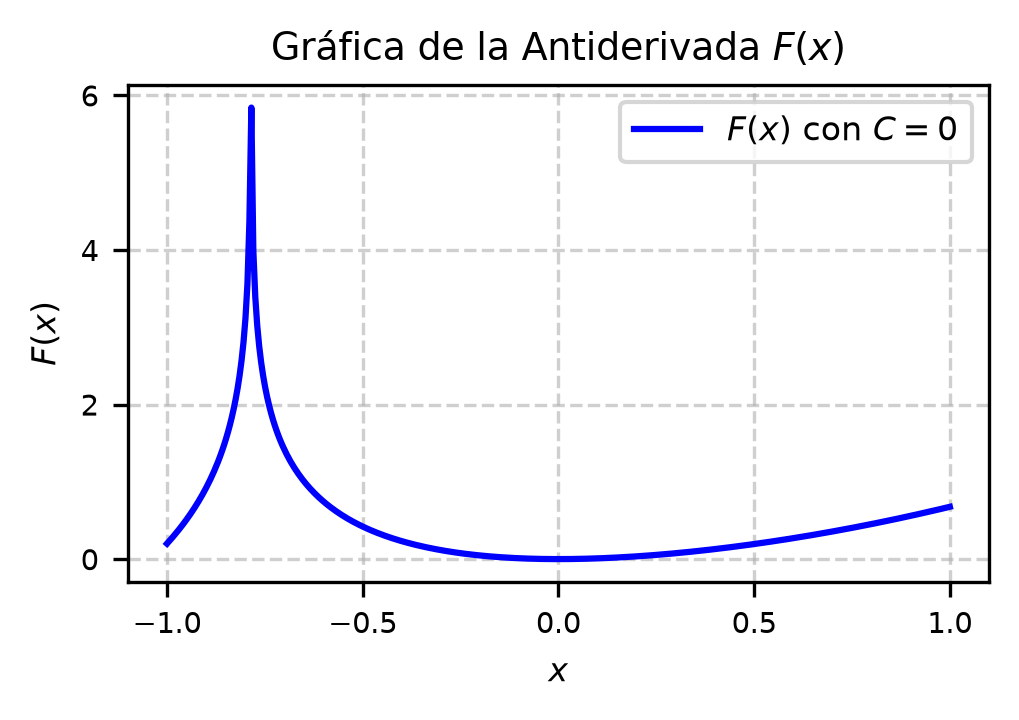
\includegraphics[width=\columnwidth]{semana_04/graficas/SEM04_P24_grafica.png}
	\caption{Representación gráfica de $f(x)$ y su antiderivada $F(x)$ evaluada para la constante de integración $C = 0$ (Problema 24).}
	\label{fig:problema24}
\end{figure}
